% Options for packages loaded elsewhere
\PassOptionsToPackage{unicode}{hyperref}
\PassOptionsToPackage{hyphens}{url}
\documentclass[
  ignorenonframetext,
  aspectratio=169]{beamer}
\newif\ifbibliography
\usepackage{pgfpages}
\setbeamertemplate{caption}[numbered]
\setbeamertemplate{caption label separator}{: }
\setbeamercolor{caption name}{fg=normal text.fg}
\beamertemplatenavigationsymbolsempty
% remove section numbering
\setbeamertemplate{part page}{
  \centering
  \begin{beamercolorbox}[sep=16pt,center]{part title}
    \usebeamerfont{part title}\insertpart\par
  \end{beamercolorbox}
}
\setbeamertemplate{section page}{
  \centering
  \begin{beamercolorbox}[sep=12pt,center]{section title}
    \usebeamerfont{section title}\insertsection\par
  \end{beamercolorbox}
}
\setbeamertemplate{subsection page}{
  \centering
  \begin{beamercolorbox}[sep=8pt,center]{subsection title}
    \usebeamerfont{subsection title}\insertsubsection\par
  \end{beamercolorbox}
}
% Prevent slide breaks in the middle of a paragraph
\widowpenalties 1 10000
\raggedbottom
\AtBeginPart{
  \frame{\partpage}
}
\AtBeginSection{
  \ifbibliography
  \else
    \frame{\sectionpage}
  \fi
}
\AtBeginSubsection{
  \frame{\subsectionpage}
}
\usepackage{iftex}
\ifPDFTeX
  \usepackage[T1]{fontenc}
  \usepackage[utf8]{inputenc}
  \usepackage{textcomp} % provide euro and other symbols
\else % if luatex or xetex
  \usepackage{unicode-math} % this also loads fontspec
  \defaultfontfeatures{Scale=MatchLowercase}
  \defaultfontfeatures[\rmfamily]{Ligatures=TeX,Scale=1}
\fi
\usepackage{lmodern}
\ifPDFTeX\else
  % xetex/luatex font selection
\fi
% Use upquote if available, for straight quotes in verbatim environments
\IfFileExists{upquote.sty}{\usepackage{upquote}}{}
\IfFileExists{microtype.sty}{% use microtype if available
  \usepackage[]{microtype}
  \UseMicrotypeSet[protrusion]{basicmath} % disable protrusion for tt fonts
}{}
\makeatletter
\@ifundefined{KOMAClassName}{% if non-KOMA class
  \IfFileExists{parskip.sty}{%
    \usepackage{parskip}
  }{% else
    \setlength{\parindent}{0pt}
    \setlength{\parskip}{6pt plus 2pt minus 1pt}}
}{% if KOMA class
  \KOMAoptions{parskip=half}}
\makeatother
\setlength{\emergencystretch}{3em} % prevent overfull lines
\providecommand{\tightlist}{%
  \setlength{\itemsep}{0pt}\setlength{\parskip}{0pt}}
% ============================================================
%  beamer_preamble.tex  (RTSL Assessment Beamer slide deck)
%  - Default Beamer look + colored callout boxes
%  - UW Purple accents for bullets/titles
%  - Custom uncertaintyblock environment
% ============================================================

% -- Beamer theme (keep default look) ----------------------------------------
\usetheme{default}
\usecolortheme{default}
\usefonttheme{professionalfonts}

% -- XeLaTeX fonts (requires xelatex engine) ----------------------------------
\usepackage{fontspec}
\setmainfont{Calibri}[
  BoldFont       = Calibri Bold,
  ItalicFont     = Calibri Italic,
  BoldItalicFont = Calibri Bold Italic
]
\setsansfont{Calibri}
\setmonofont{Courier New}

% -- Packages -----------------------------------------------------------------
\usepackage{booktabs}
\usepackage{xcolor}
\usepackage{soul}
\usepackage{colortbl}
\usepackage{array}
\usepackage{graphicx}
\usepackage{ragged2e}
\usepackage{longtable}
\usepackage{tabu}
\usepackage{microtype}
\usepackage{hyperref}
\usepackage{tikz}

% -- Larger default font for donor/funder audience ----------------------------
% Presentation is delivered live; increase base font size for readability.
\setbeamerfont{normal text}{size=\large}
\setbeamerfont{title}{size=\huge,series=\bfseries}
\setbeamerfont{subtitle}{size=\Large}
\setbeamerfont{frametitle}{size=\LARGE,series=\bfseries}
\setbeamerfont{framesubtitle}{size=\large}
\setbeamerfont{block title}{size=\large,series=\bfseries}
\setbeamerfont{block title alerted}{size=\large,series=\bfseries}
\setbeamerfont{block title example}{size=\large,series=\bfseries}
\setbeamerfont{itemize/enumerate body}{size=\large}
\setbeamerfont{itemize/enumerate subbody}{size=\normalsize}
\setbeamerfont{caption}{size=\small}
\AtBeginDocument{\large}

% -- Project colour palette ---------------------------------------------------
\definecolor{uwpurple}{HTML}{4B2E83}
\definecolor{uwgold}{HTML}{85754D}
\definecolor{rtslblue}{HTML}{2171B5}
\definecolor{rtslgreen}{HTML}{74C476}
\definecolor{rtslred}{HTML}{E31A1C}
\definecolor{rtslpurple}{HTML}{6A3D9A}
\definecolor{baugrey}{HTML}{999999}
\definecolor{highlightblue}{HTML}{DBEAFE}
\definecolor{uncertaintyyellow}{HTML}{FFF3CD}
\definecolor{uncertaintyborder}{HTML}{856404}

% -- Title & structure colors -------------------------------------------------
\setbeamercolor{structure}{fg=uwpurple}
\setbeamercolor{title}{fg=uwpurple}
\setbeamercolor{subtitle}{fg=uwpurple}
\setbeamercolor{author}{fg=black}
\setbeamercolor{date}{fg=black}
\setbeamercolor{institute}{fg=black}
\setbeamercolor{frametitle}{fg=uwpurple}
\setbeamercolor{normal text}{fg=black}

% -- Colored blocks (callout boxes) -------------------------------------------
% block = theme color (definitions)
\setbeamercolor{block title}{bg=baugrey!15, fg=black}
\setbeamercolor{block body}{bg=baugrey!6}

% alertblock = red (open questions / pending decisions)
\setbeamercolor{block title alerted}{bg=red!15, fg=red!70!black}
\setbeamercolor{block body alerted}{bg=red!6}

% exampleblock = green (key takeaways)
\setbeamercolor{block title example}{bg=rtslgreen!18, fg=rtslgreen!80!black}
\setbeamercolor{block body example}{bg=rtslgreen!6}

% Custom: uncertaintyblock = amber (uncertainties / sensitivity caveats)
\newenvironment{uncertaintyblock}[1]{%
  \setbeamercolor{block title}{bg=uncertaintyyellow, fg=uncertaintyborder}%
  \setbeamercolor{block body}{bg=uncertaintyyellow!30}%
  \begin{block}{#1}%
}{\end{block}}

% -- Bullet style -------------------------------------------------------------
\setbeamertemplate{itemize item}{\textcolor{uwpurple}{\textbullet}}
\setbeamertemplate{itemize subitem}{\textcolor{uwpurple}{--}}
\setbeamertemplate{enumerate item}{\textcolor{uwpurple}{\insertenumlabel.}}

% -- Footer -------------------------------------------------------------------
% \setbeamertemplate{footline}{%
%   \leavevmode
%   \hbox{%
%     \begin{beamercolorbox}[wd=0.45\paperwidth, ht=2.25ex, dp=1ex, left]{author in head/foot}%
%       \hspace{1em}\usebeamerfont{author in head/foot}%
%       \textcolor{black!60}{\footnotesize RTSL -- UW Assessment}%
%     \end{beamercolorbox}%
%     \begin{beamercolorbox}[wd=0.45\paperwidth, ht=2.25ex, dp=1ex, center]{title in head/foot}%
%       \usebeamerfont{title in head/foot}%
%       \textcolor{black!60}{\footnotesize CVD Program Impact}%
%     \end{beamercolorbox}%
%     \begin{beamercolorbox}[wd=0.10\paperwidth, ht=2.25ex, dp=1ex, right]{date in head/foot}%
%       \usebeamerfont{date in head/foot}%
%       \textcolor{black!60}{\footnotesize \insertframenumber{}/\inserttotalframenumber}%
%       \hspace{0.5em}%
%     \end{beamercolorbox}%
%   }%
%   \vskip0pt%
% }
\setbeamertemplate{navigation symbols}{}

% -- UW logo in bottom-right corner of every slide ----------------------------
% Uses tikz overlay so logo floats in the corner without pushing content.
% Reserve a small bottom margin via footline to avoid overlap with slide body.
\setbeamertemplate{footline}{%
  \leavevmode\vspace*{0.9cm}%
}

\addtobeamertemplate{background canvas}{}{%
  \begin{tikzpicture}[remember picture, overlay]
    \node[anchor=south east, xshift=-0.25cm, yshift=0.2cm]
      at (current page.south east)
      {
\includegraphics[height=0.65cm,keepaspectratio]{uw-logo.png}};
  \end{tikzpicture}%
}

% -- Section slide (auto-generated by # headers) ------------------------------
\AtBeginSection[]{%
  \begin{frame}
    \vfill
    \centering
    \begin{beamercolorbox}[sep=8pt, center, shadow=false, rounded=true]{block title}
      \usebeamerfont{title}\insertsectionhead\par
    \end{beamercolorbox}
    \vfill
  \end{frame}
}
\usepackage{booktabs}
\usepackage{longtable}
\usepackage{array}
\usepackage{multirow}
\usepackage{wrapfig}
\usepackage{float}
\usepackage{colortbl}
\usepackage{pdflscape}
\usepackage{tabu}
\usepackage{threeparttable}
\usepackage{threeparttablex}
\usepackage[normalem]{ulem}
\usepackage{makecell}
\usepackage{xcolor}
\usepackage{bookmark}
\IfFileExists{xurl.sty}{\usepackage{xurl}}{} % add URL line breaks if available
\urlstyle{same}
\hypersetup{
  pdftitle={RTSL Cardiovascular Health Program Impact},
  pdfauthor={University of Washington -- Resolve to Save Lives},
  hidelinks,
  pdfcreator={LaTeX via pandoc}}

\title{RTSL Cardiovascular Health Program Impact}
\subtitle{Projected health outcomes across RTSL-engaged countries,
2017--2050}
\author{University of Washington -- Resolve to Save Lives}
\date{April 2026}

\begin{document}
\frame{\titlepage}

\begin{frame}
\end{frame}

\begin{frame}{Setting the Stage}
\phantomsection\label{setting-the-stage}
\begin{columns}[T]
\begin{column}{0.32\textwidth}
\textbf{\color{uwpurple}What is the problem?}
\vspace{0.2em}

\footnotesize
\begin{itemize}
  \item \textbf{Hypertension} and \textbf{industrially-produced trans fat} are two of the most preventable drivers of cardiovascular disease.
  \item Together, they account for millions of premature deaths every year.
\end{itemize}
\scriptsize \textit{Sources: GBD 2023 (IHME); WHO Global Report on Hypertension.}
\end{column}

\begin{column}{0.32\textwidth}
\textbf{\color{uwpurple}Why does it matter?}
\vspace{0.2em}

\footnotesize
\begin{itemize}
  \item CVD causes \textbf{19.2 million} deaths each year globally --- approximately one-third of all deaths.
  \item High blood pressure alone drives \textbf{10.8 million} deaths annually.
  \item Trans fat adds another \textbf{500,000} IHD deaths.
\end{itemize}
\scriptsize \textit{Sources: Lancet 2025; WHO; GBD 2023.}
\end{column}

\begin{column}{0.32\textwidth}
\textbf{\color{uwpurple}Who is affected?}
\vspace{0.2em}

\footnotesize
\begin{itemize}
  \item \textbf{over 80\%} of CVD deaths occur in low- and middle-income countries.
  \item \textbf{over three-quarters} of \textit{premature} CVD deaths are in LMICs.
  \item Populations without access to treatment or policy protection bear the greatest burden.
\end{itemize}
\scriptsize \textit{Sources: Lancet 2025; WHO.}
\end{column}
\end{columns}
\end{frame}

\begin{frame}[fragile]{The Challenge in Numbers}
\phantomsection\label{the-challenge-in-numbers}
\begin{columns}[T]
\begin{column}{0.48\textwidth}
\textbf{\color{uwpurple}Hypertension}
\vspace{0.4em}

{\huge \textbf{1.3 billion}} \newline
\small adults live with hypertension worldwide

\vspace{0.5em}
{\huge \textbf{over 75\%}} \newline
\small of them are not controlled

\vspace{0.5em}
{\huge \textbf{nearly half}} \newline
\small are undiagnosed

\vspace{0.8em}
\scriptsize \textit{WHO Global Report on Hypertension (2023/2025 update); resolvetosavelives.org/blood-pressure-control.}
\end{column}

\begin{column}{0.48\textwidth}
\textbf{\color{uwpurple}Trans fat}
\vspace{0.4em}

{\huge \textbf{67}} \newline
\small countries with WHO best-practice TFA policies

\vspace{0.5em}
{\huge \textbf{roughly 5 billion}} \newline
\small people still unprotected

\vspace{0.5em}
{\huge \textbf{500,000}} \newline
\small IHD deaths every year from industrial trans fat

\vspace{0.8em}
\scriptsize \textit{WHO REPLACE; resolvetosavelives.org/healthier-food.}
\end{column}
\end{columns}
\end{frame}

\begin{frame}{What RTSL Does}
\phantomsection\label{what-rtsl-does}
\justifying

RTSL collaborates with governments and other partners in more than 76
countries to deliver proven, scalable CVH interventions:

\medskip

\begin{itemize}
\tightlist
\item
  \textbf{Hypertension control} --- blood pressure screening, treatment,
  and follow-up programs reaching millions of patients since 2017
\item
  \textbf{Trans-fat elimination} --- technical assistance and advocacy
  to enact and implement best-practice policies that remove industrial
  trans fats from the food supply
\item
  \textbf{Targeting the highest-risk populations} with the most
  cost-effective interventions available
\end{itemize}
\end{frame}

\begin{frame}[fragile]{Our Approach}
\phantomsection\label{our-approach}
\begin{columns}[T]
\begin{column}{0.32\textwidth}
\textbf{\color{uwpurple}What we did}
\vspace{0.2em}

\footnotesize
\begin{itemize}
  \item Built a country-level, multi-state CVD simulation across 76 countries.
  \item Projected deaths averted from 2017 to 2050 under observed RTSL program and policy trajectories.
  \item Combined HTN control and TFA elimination into one integrated assessment.
\end{itemize}
\end{column}

\begin{column}{0.32\textwidth}
\textbf{\color{uwpurple}Who we worked with}
\vspace{0.2em}

\footnotesize
\begin{itemize}
  \item \textbf{Resolve to Save Lives} --- program, policy, and country teams.
  \item \textbf{Country governments and ministries of health} providing program data.
  \item \textbf{WHO} (REPLACE, HEARTS) policy frameworks and data.
  \item \textbf{IHME / GBD} for baseline epidemiology.
\end{itemize}
\end{column}

\begin{column}{0.32\textwidth}
\textbf{\color{uwpurple}How it was implemented}
\vspace{0.2em}

\footnotesize
\begin{itemize}
  \item Country-by-country modeling using RTSL monitoring data (2017--2025) and UNWPP 2024 projections.
  \item Scenario analysis: program vs. counterfactual, for each intervention.
  \item Results reviewed with RTSL and country partners.
\end{itemize}
\end{column}
\end{columns}
\end{frame}

\begin{frame}[fragile]{Headline Impact: 9.6 Million Lives Saved}
\phantomsection\label{headline-impact-9.6-million-lives-saved}
\justifying

\medskip

Across \textbf{76 countries}, RTSL cardiovascular health programs are
projected to avert \textbf{9.6 deaths} from 2017--2050, combining
hypertension control and trans-fat elimination.

\medskip

That is approximately \textbf{772 deaths averted every day} over more
than three decades.

\medskip

\begin{exampleblock}{What This Means}
Sustained investment in hypertension control and trans-fat elimination is projected to deliver one of the largest preventable reductions in cardiovascular mortality across RTSL-engaged countries.
\end{exampleblock}
\end{frame}

\begin{frame}{Where Impact Is Concentrated}
\phantomsection\label{where-impact-is-concentrated}
\begin{center}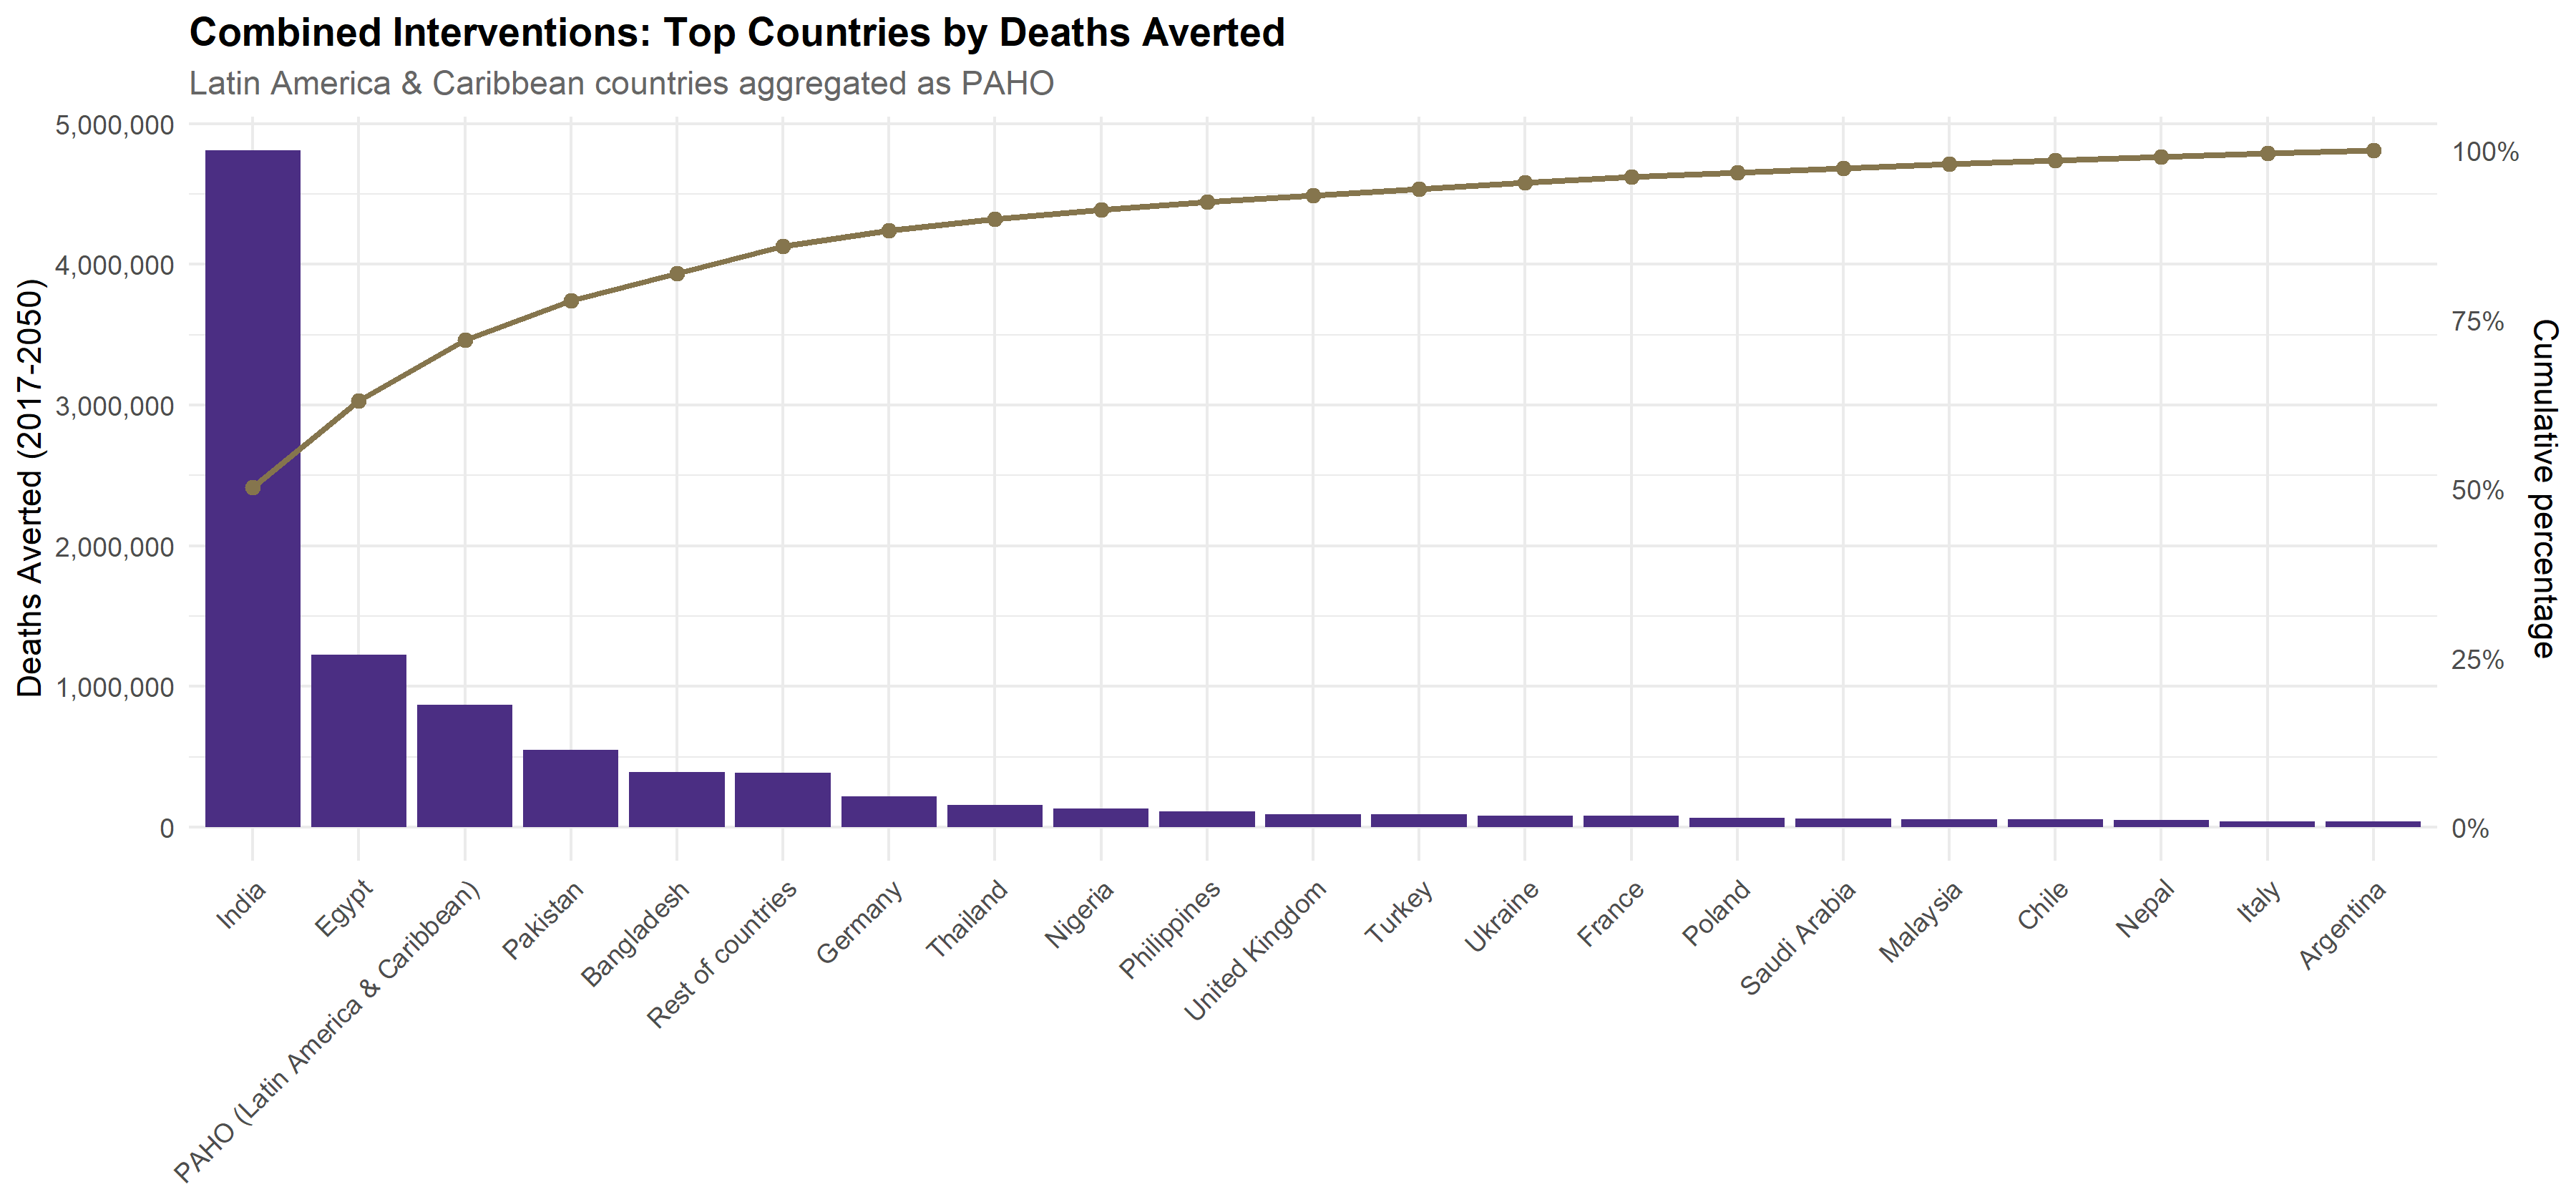
\includegraphics[width=\linewidth]{presentation_cvh_partners_donors_files/figure-beamer/pareto-combined-paho-1} \end{center}

\footnotesize  Top 20 entries. All Latin America and Caribbean countries
combined into a single ``PAHO'' bar.
\end{frame}

\begin{frame}{Global Coverage: HTN and TFA Interventions}
\phantomsection\label{global-coverage-htn-and-tfa-interventions}
\begin{center}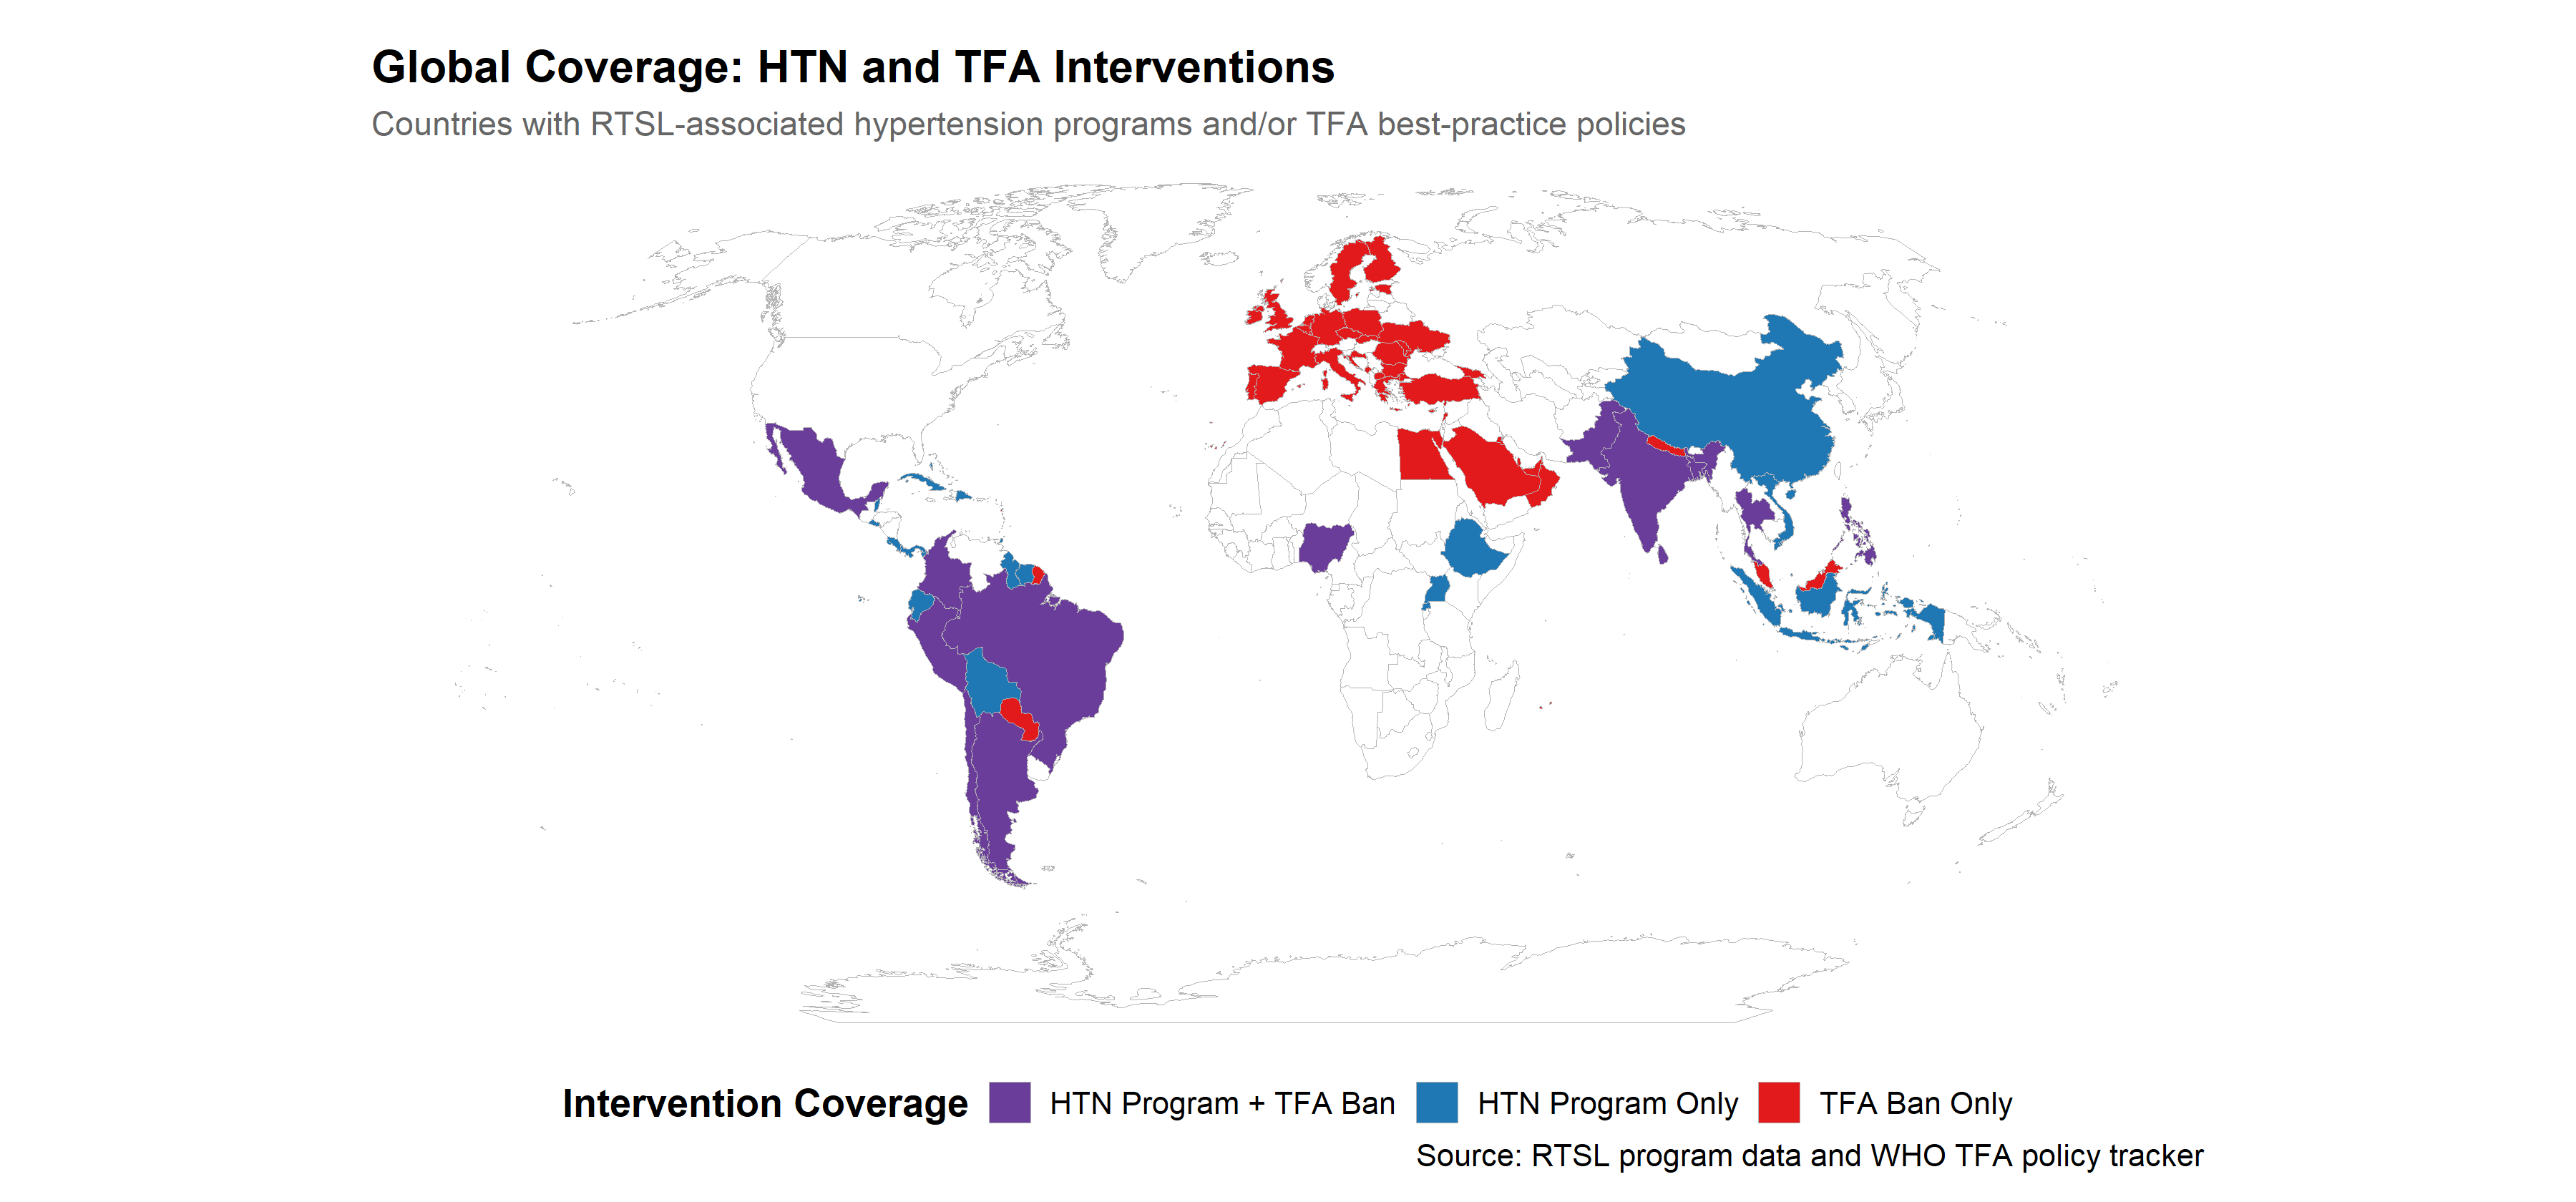
\includegraphics[width=\linewidth]{presentation_cvh_partners_donors_files/figure-beamer/fig-country-map-1} \end{center}
\end{frame}

\begin{frame}{Trans Fat Elimination: Global Policy Progress}
\phantomsection\label{trans-fat-elimination-global-policy-progress}
\begin{center}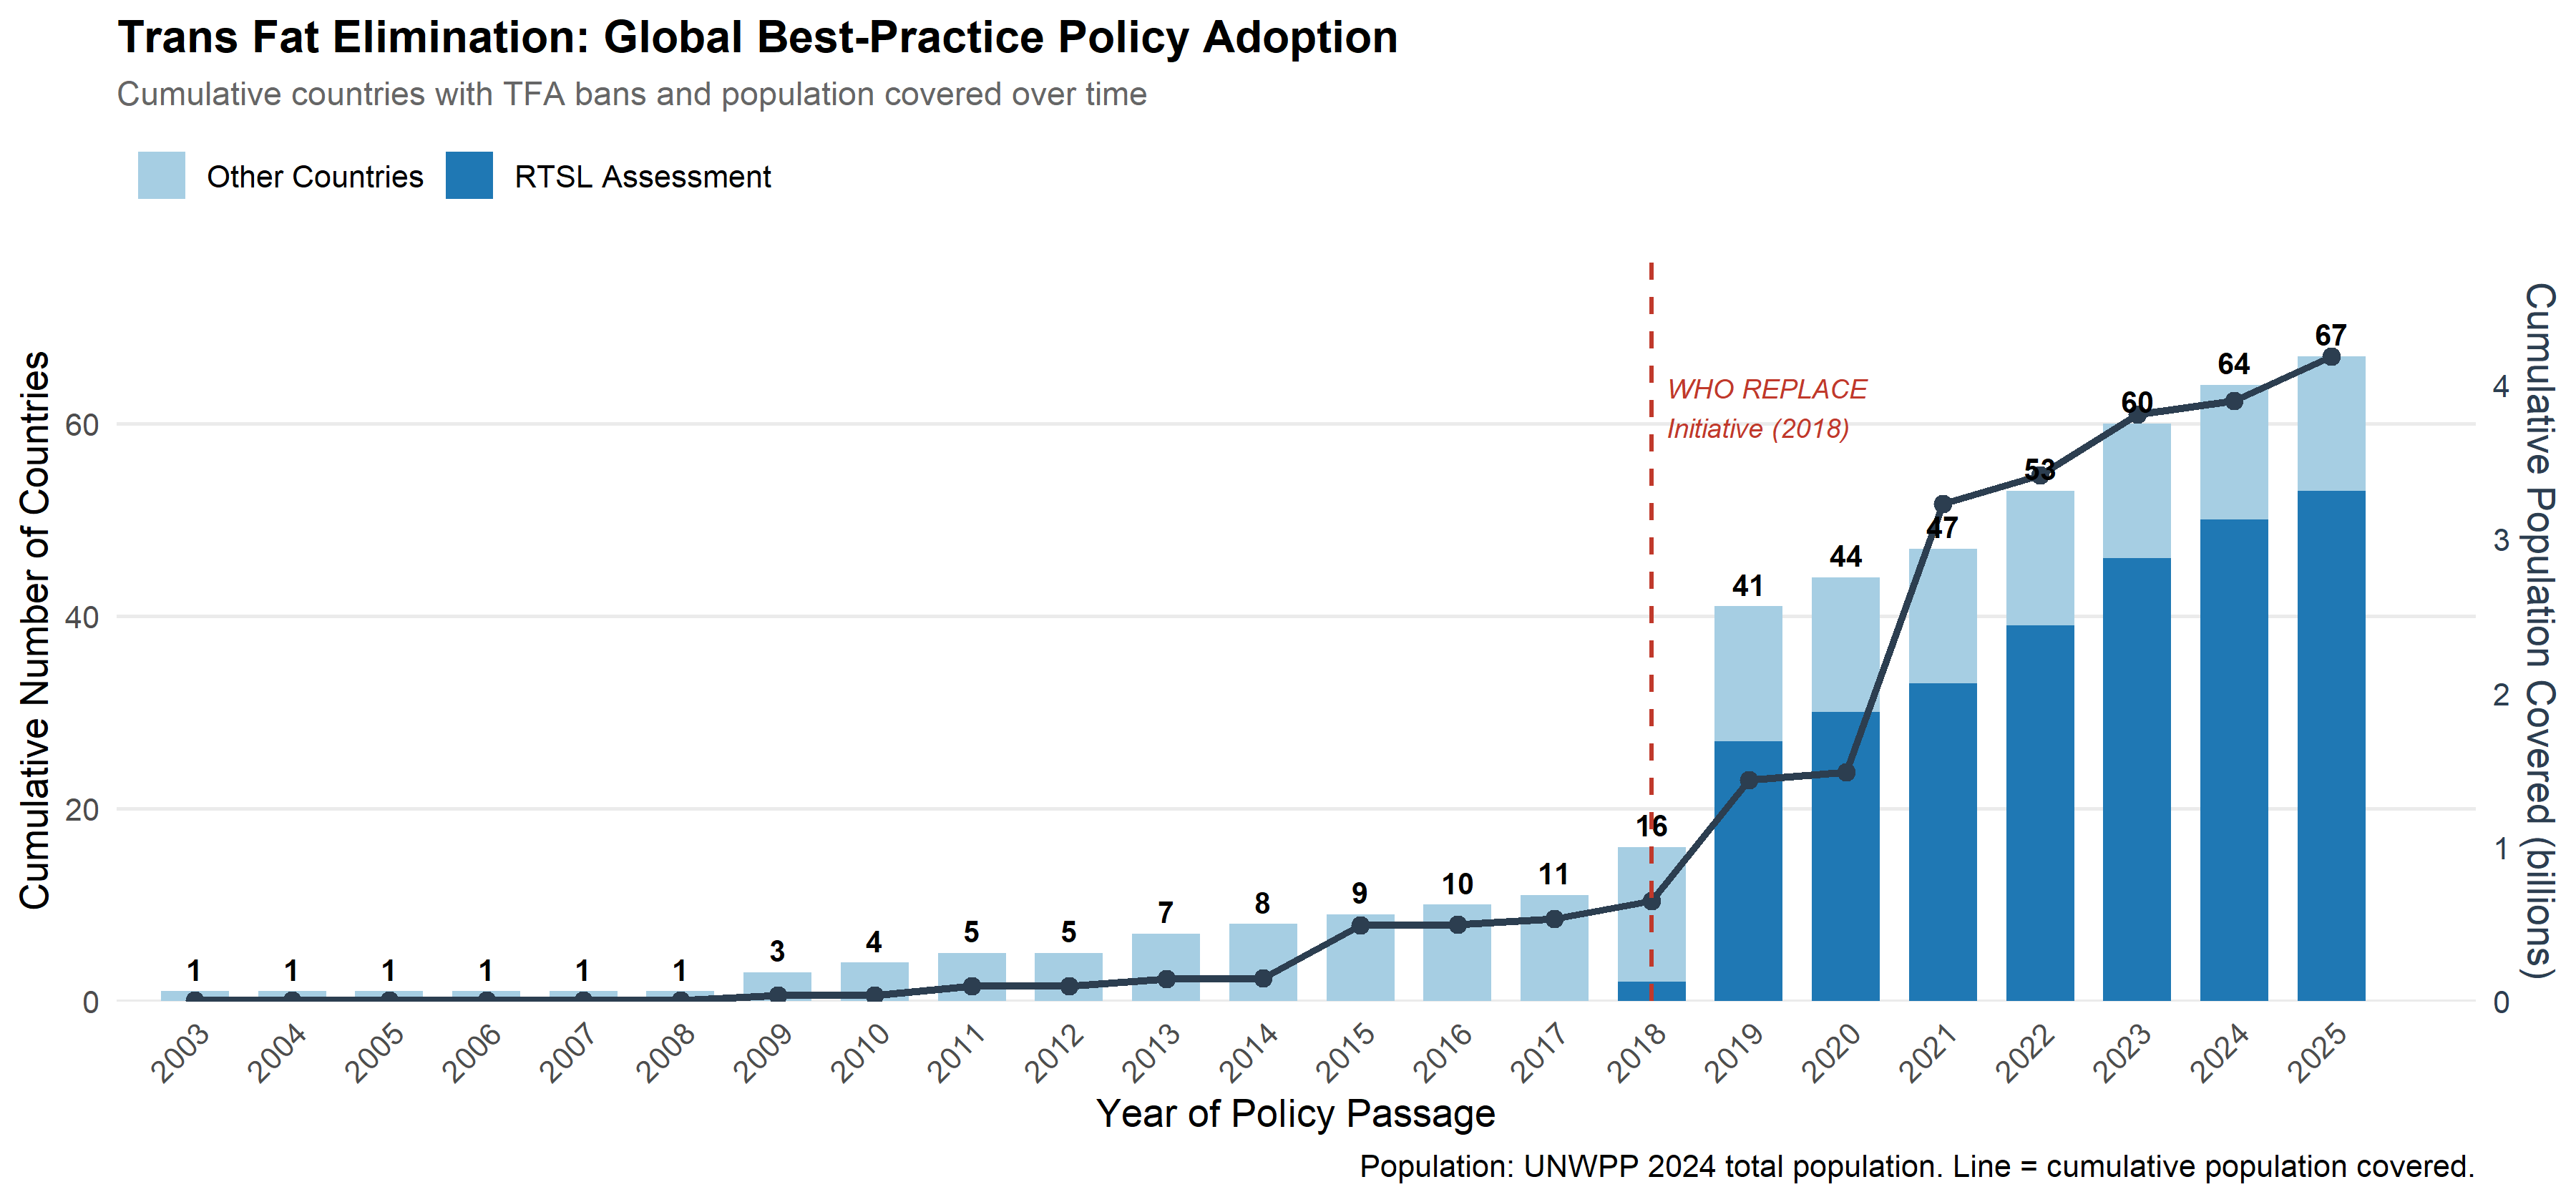
\includegraphics[width=\linewidth]{presentation_cvh_partners_donors_files/figure-beamer/fig-tfa-timeline-1} \end{center}
\end{frame}

\begin{frame}{RTSL Hypertension Program Enrollment Over Time}
\phantomsection\label{rtsl-hypertension-program-enrollment-over-time}
\begin{center}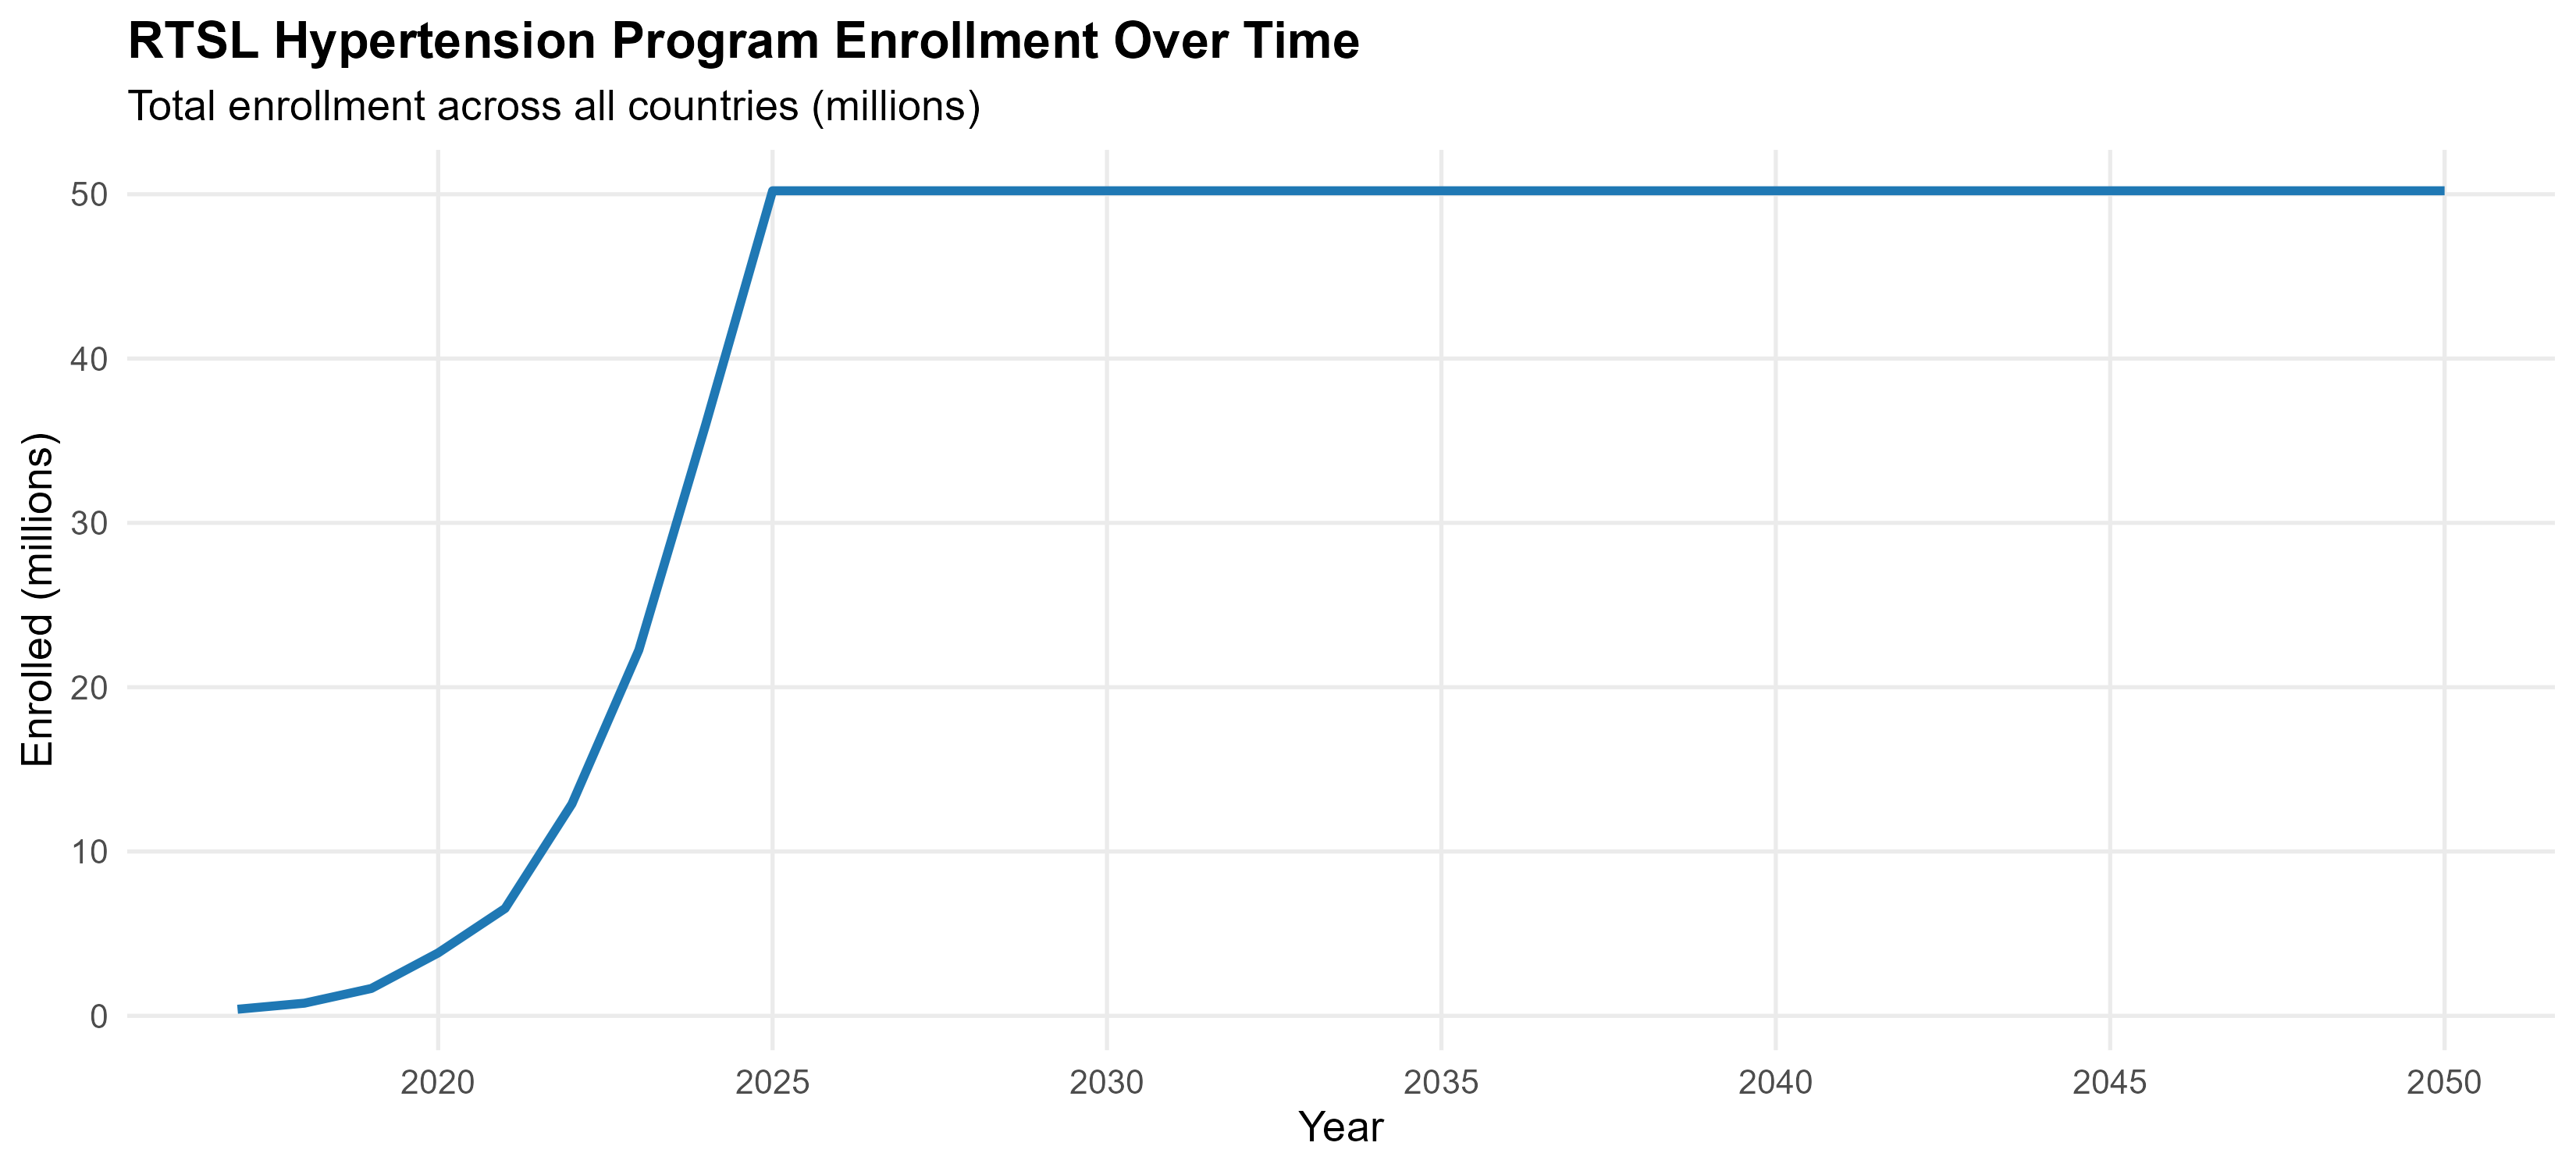
\includegraphics[width=0.9\linewidth]{../output/assessment_enrollment_trend} \end{center}

\footnotesize Enrollment and program-controlled population. Post-2025
values held constant at 2025 observed levels.
\end{frame}

\begin{frame}[fragile]{What We Learned}
\phantomsection\label{what-we-learned}
\begin{columns}[T]
\begin{column}{0.48\textwidth}
\textbf{\color{uwpurple}What surprised us}
\footnotesize
\begin{itemize}
  \item A small number of countries drive most of the global impact: scale of the program matters as much as its efficacy.
\end{itemize}

\medskip
\textbf{\color{uwpurple}What we would do differently}
\footnotesize
\begin{itemize}
  \item Pair modeling more closely with real-time program data feeds.
  \item Invest earlier in a shared data dictionary across country teams.
\end{itemize}
\end{column}

\begin{column}{0.48\textwidth}
\textbf{\color{uwpurple}Barriers we encountered}
\footnotesize
\begin{itemize}
  \item Uneven and delayed country reporting on BP control and program enrollment.
  \item Heterogeneous TFA policy data (passage vs. enforcement dates).
  \item Baseline CVD epidemiology shifts between GBD releases.
  \item Counterfactual definition is contested --- small methodological choices move totals substantially.
\end{itemize}
\end{column}
\end{columns}
\end{frame}

\begin{frame}[fragile]{What's Next}
\phantomsection\label{whats-next}
\footnotesize
\begin{itemize}
  \item \textbf{Extend} the modeling framework to additional RTSL priority countries and to secondary risk factors (sodium).
  \item \textbf{Refresh} country estimates on an annual cadence as program and policy data arrive.
  \item \textbf{Translate} findings into a country-facing, interactive tool for ministries of health and partners.
  \item \textbf{Disseminate} results through peer-reviewed publication and global health forums to inform policy and funding decisions. "100 Million Lives Saved" manuscript currently under review.
\end{itemize}

\medskip

\begin{exampleblock}{One ask}
\large Help us turn 9.6 million projected lives saved into a shared, actionable evidence base for ministries, donors, and advocates.
\end{exampleblock}
\end{frame}

\section{Extra Slides}\label{extra-slides}

\begin{frame}[fragile]{Methodology at a Glance}
\phantomsection\label{methodology-at-a-glance}
\begin{columns}[T]
\begin{column}{0.48\textwidth}
\textbf{\color{uwpurple}Model structure}
\footnotesize
\begin{itemize}
  \item Discrete-time, country-by-country multi-state model (Well $\rightarrow$ Sick $\rightarrow$ Dead), ages 20--95, 2017--2050.
  \item Four CVD causes modeled: IHD, ischemic stroke, intracerebral hemorrhage, hypertensive heart disease.
  \item Baseline rates from GBD 2023 (IHME); population from UNWPP 2024.
\end{itemize}
\end{column}

\begin{column}{0.48\textwidth}
\textbf{\color{uwpurple}Interventions and counterfactual}
\footnotesize
\begin{itemize}
  \item \textbf{HTN:} observed RTSL program control rates (2017--2025) maintained to 2050; Ettehad et al. 2016 treatment effects.
  \item \textbf{TFA:} full elimination of industrial TFA in countries with enacted best-practice policies.
  \item \textbf{Counterfactual:} zero incremental program effect (business-as-usual).
  \item \textbf{Combined:} HTN and TFA filtered separately (different target populations), then summed per country.
\end{itemize}
\end{column}
\end{columns}

\vspace{0.4em}

\footnotesize \textit{Inputs: GBD 2023, GBD 2019 RRs, UNWPP 2024, HTN Global Tracker, WHO TFA policy tracker, RTSL program monitoring data.}
\end{frame}

\end{document}
